This section details the interfaces between the Best Bike Paths (BBP) system and external entities, including users, hardware components, other software systems, and communication networks. These interfaces define how BBP interacts with its operational environment.
\section{External interface requirements}
\label{sec:external_interface_requirements}%

\subsection{User interfaces}
\label{subsec:User_interfaces}%
The primary user interface for the BBP system will be a native mobile application designed for smartphones (iOS and Android platforms). The interface must prioritize clarity, usability, and robustness, particularly for outdoor use under varying light conditions. It will adopt a map-centric design, prominently displaying geographical data and route information. Key interaction elements will include a clear search bar for origin/destination input, interactive map elements for manual route creation and viewing details, easily accessible buttons for critical functions like starting/stopping automatic recording, and a dedicated Heads-Up Display (HUD) during active recording sessions showing real-time statistics (speed, distance, time) with high legibility. The interface will also incorporate clear feedback mechanisms and prompts for user input, such as the review and confirmation of automatically detected sensor events presented at the conclusion of a trip . Navigation between different sections (e.g., Map, Search Results, My Trips, User Profile) must be intuitive and consistent throughout the application.
\subsection{Hardware interfaces}
\label{subsec:hardware_interfaces}%
The BBP system requires direct interaction with specific hardware components integral to the user's mobile device. Foremost is the Global Positioning System (GPS) receiver, from which the application must continuously acquire accurate location data (latitude, longitude, timestamp) to track the user's position during navigation and automatic trip recording. Secondly, BBP must interface with the device's inertial measurement unit (IMU) sensors, specifically the accelerometer and gyroscope. Access to the raw data streams from these sensors is mandatory for the implementation of the automatic obstacle detection feature, enabling BBP to identify significant motion events that may correspond to real-world path anomalies, such as potholes. Furthermore, the application relies on standard smartphone hardware, including the touchscreen display for all user input and output, and potentially the device's vibration motor for non-visual notifications (e.g., indicating a potential obstacle has been logged). BBP assumes these hardware components are functional and accessible via the device's operating system APIs.

\subsection{Software interfaces}
\label{subsec:software_interfaces}%
BBP will interact with several other software entities. A critical interface exists with the mobile device's Operating System (OS). Through OS APIs, BBP must request and manage permissions for accessing hardware sensors (GPS, accelerometer, gyroscope), handle background execution for continuous trip recording, potentially manage local storage for application data, and interact with network services. Another vital software interface is with the External Weather Service. BBP must communicate with this external service via its provided Application Programming Interface (API), likely transmitting location coordinates (and potentially time information) and receiving structured weather forecast data (e.g., in JSON format) containing temperature, wind speed, precipitation probability, and general conditions . The specific protocol and data format will be dictated by the chosen weather service provider. 

\subsection{Communication interfaces}
\label{subsec:communication_interfaces}%

The BBP system inherently requires network connectivity for many of its core functions. An active internet connection, typically via cellular data (e.g., 4G, 5G) or Wi-Fi, is necessary for user authentication (signup/login), searching for public paths, retrieving path details (including merged status and reports) , fetching real-time weather data from the external service , and saving or publishing user-generated trips and reports. Communication with the BBP backend server (which manages user accounts, paths, reports, etc.) will occur over standard secure web protocols(HTTPS), to ensure data integrity and confidentiality during transit. BBP must gracefully handle temporary losses of connectivity where possible, although core online features will be unavailable without an active connection (as per DA12).
\section{Functional requirements}
\label{sec:functional_requirements}%

\subsection{Requirements}
\label{subsec:requirements3}%
\newcounter{reqcounter} % Create a counter for requirements
\renewcommand{\thereqcounter}{R\arabic{reqcounter}} % Define the format R1, R2...

This section lists the specific functional requirements that the Best Bike Paths (BBP) system must fulfill.


% Required packages (ensure these are in your preamble)
% \usepackage{longtable}
% \usepackage{array}

% Counter definition (ensure this is in your preamble)
% \newcounter{reqcounter}
% \renewcommand{\thereqcounter}{R\arabic{reqcounter}}

\begin{longtable}{|p{0.1\textwidth}|p{0.8\textwidth}|}
\hline
\textbf{ID} & \textbf{Description} \\ 
\hline
\endfirsthead

\hline
\textbf{ID} & \textbf{Description} \\ 
\hline
\endhead

\hline \multicolumn{2}{r|}{{Continued on next page}} \\
\endfoot

\hline
\endlastfoot

% --- User Management ---


% --- User Management ---
\setcounter{reqcounter}{0} % Reset counter just before the first data row
\stepcounter{reqcounter} \thereqcounter & BBP allows Users to sign up \\
\hline
\stepcounter{reqcounter} \thereqcounter & BBP shall verify that the username and email provided during registration are not already in use. \\
\hline
 \stepcounter{reqcounter} \thereqcounter & BBP shall allow RCY to log in using their username/email and password. \\
\hline
 \stepcounter{reqcounter} \thereqcounter & BBP shall provide feedback to the user in case of failed login attempts (e.g., incorrect credentials). \\
\hline
\stepcounter{reqcounter} \thereqcounter & BBP shall allow an RCY to view the personal page with private information. \\
\hline
 \stepcounter{reqcounter} \thereqcounter & BBP shall allow a logged-in user to log out. \\
\hline

% --- Path Discovery & Navigation ---
 \stepcounter{reqcounter} \thereqcounter & BBP shall allow any user to search for public bike paths by specifying an origin and a destination. \\
\hline
 \stepcounter{reqcounter} \thereqcounter & BBP shall retrieve all relevant \texttt{Report} instances associated with the paths found during a search. \\
\hline
 \stepcounter{reqcounter} \thereqcounter & BBP shall calculate a merged status for each searched path based on its associated \texttt{Status\_report} instances, applying freshness and majority rules. \\
\hline
 \stepcounter{reqcounter} \thereqcounter & BBP shall calculate a score for each searched path based on its reports/conditions and metrics. \\
\hline
 \stepcounter{reqcounter} \thereqcounter & BBP shall display search results as a list of paths ordered by the calculated score. \\
\hline
 \stepcounter{reqcounter} \thereqcounter & BBP shall allow any user to select a path from the search results to view its details. \\
\hline
 \stepcounter{reqcounter} \thereqcounter & BBP shall display the details of a selected path, including its geometry (map), distance, elevation, calculated merged status, and reported obstacles. \\
\hline
 \stepcounter{reqcounter} \thereqcounter & BBP shall retrieve and display current weather forecast information for the selected path's location. \\
\hline
 \stepcounter{reqcounter} \thereqcounter & BBP shall allow any user to initiate a navigation mode ("Follow Route") for a selected path. \\
\hline
 \stepcounter{reqcounter} \thereqcounter & Upon completion of navigation by a user, BBP shall show the summary of the trip (example: avg. speed, distance,...). \\
\hline
 \stepcounter{reqcounter} \thereqcounter & Upon completion of navigation by an anonymous user, BBP shall offer the option to register. \\
\hline
 \stepcounter{reqcounter} \thereqcounter & If an anonymous user refuses registration after navigation, BBP shall discard the navigation session data. \\
\hline
 \stepcounter{reqcounter} \thereqcounter & If an anonymous user accepts registration after navigation, BBP shall allow them to complete registration and then save the navigated session as a \texttt{Trip}. \\
\hline

% --- Trip Recording & Management ---
 \stepcounter{reqcounter} \thereqcounter & BBP shall allow an RCY to start an automatic trip recording session. \\
\hline
 \stepcounter{reqcounter} \thereqcounter & During automatic recording, BBP shall record the user's GPS coordinates sequence. \\
\hline
 \stepcounter{reqcounter} \thereqcounter & During automatic recording, BBP shall display real-time statistics (speed, distance, time). \\
\hline
 \stepcounter{reqcounter} \thereqcounter & During automatic recording, a system shall monitor accelerometer and gyroscope data. \\
\hline
 \stepcounter{reqcounter} \thereqcounter & BBP shall internally log a \texttt{sensor\_event} when sensor data exceeds a predefined threshold. \\
\hline
 \stepcounter{reqcounter} \thereqcounter & BBP shall allow an RCY to stop the automatic trip recording. \\
\hline
 \stepcounter{reqcounter} \thereqcounter & Upon stopping recording, if \texttt{sensor\_event}s were logged, BBP shall present them to the user for review. \\
\hline
 \stepcounter{reqcounter} \thereqcounter & BBP shall allow the user to confirm or ignore each \texttt{sensor\_event} during review. \\
\hline
 \stepcounter{reqcounter} \thereqcounter & BBP shall create an \texttt{Obstacle\_report} associated with the trip only for confirmed \texttt{sensor\_event}s. \\
\hline
 \stepcounter{reqcounter} \thereqcounter & After recording (and review), BBP shall calculate final trip statistics. \\
\hline
 \stepcounter{reqcounter} \thereqcounter & After recording, BBP shall retrieve and associate weather information with the trip. \\
\hline
 \stepcounter{reqcounter} \thereqcounter & BBP shall allow the user to save the completed \texttt{Trip} (path, stats, weather, confirmed reports) to their private archive. \\
\hline
 \stepcounter{reqcounter} \thereqcounter & BBP shall allow an RCY to view their list of saved trips. \\
\hline
 \stepcounter{reqcounter} \thereqcounter & BBP shall allow an RCY to view the details of a saved trip. \\
\hline
 \stepcounter{reqcounter} \thereqcounter & BBP shall allow an RCY to delete a saved trip. \\
\hline
 \stepcounter{reqcounter} \thereqcounter & BBP shall allow an RCY, after they have saved the trip, to make it public the path \\
\hline

% --- Manual Creation & Reporting ---
 \stepcounter{reqcounter} \thereqcounter & BBP shall provide an editor for RCY to manually create a path geometry on a map. \\
\hline
 \stepcounter{reqcounter} \thereqcounter & BBP shall allow RCY to submit \texttt{Status\_report}s manually for paths. \\
\hline
 \stepcounter{reqcounter} \thereqcounter & BBP shall allow RCY to submit \texttt{Obstacle\_report}s manually for paths. \\
\hline
 \stepcounter{reqcounter} \thereqcounter & BBP shall allow an RCY to specify the visibility (Public/Private) when saving a trip or manually created path. \\
\hline


% --- General ---
 \stepcounter{reqcounter} \thereqcounter & BBP shall display feedback messages (confirmations, errors) to the user. \\
\hline

\end{longtable}
\subsection{Use case diagrams}
\label{subsec:use_case_diagrams}%


\begin{figure}[H]
    \begin{center}
        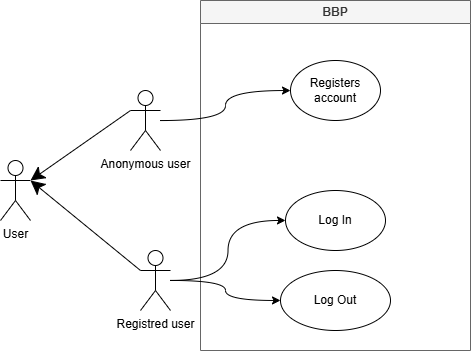
\includegraphics[width=1\linewidth]{RASD/LaTeXCode/images/useCaseDiagrams/Use_Case_1.drawio.png}
        \caption{Use Cases Diagram for  Users.} 
        \label{fig:}%
    \end{center}
\end{figure}



\begin{figure}[H]
    \begin{center}
        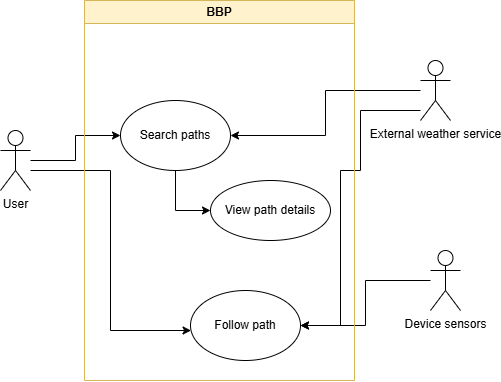
\includegraphics[width=1\linewidth]{RASD/LaTeXCode/images/useCaseDiagrams/Use_Case_2.drawio.png}
        \caption{Use Cases Diagram for bot ACY and RCY (general user).}
        \label{fig:}%
    \end{center}
\end{figure}



\begin{figure}[H]
    \begin{center}
        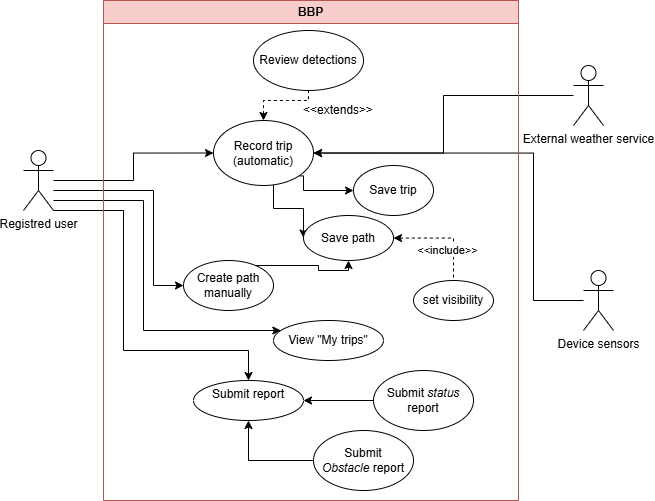
\includegraphics[width=1\linewidth]{RASD/LaTeXCode/images/useCaseDiagrams/Use_Case_3.drawio.png}
        \caption{Use Cases Diagram for RCY}
        \label{fig:}%
    \end{center}
\end{figure}

\newpage
\subsubsection{Use cases and sequence diagrams}
\label{subsec: use_cases_and_sequence_diagrams}%
 In this section, they are explained and represented the main identi ed use cases.
 There is a table with entry conditions, event ow, exit conditions and exception for each
 of them, and a sequence diagram that shows the messages exchanged between the entities
 and the called functions

\newcounter{uc}
\setcounter{uc}{1}
\newcommand{\cuc}{\theuc\stepcounter{uc}}


\subsubsection*{[UC\cuc]. Register Account}
\begin{center}
    \begin{longtable}{|l|p{0.75\linewidth}|}
        \hline
        \textbf{Actor}            & Anonymous User \\
        \hline
        \textbf{Entry conditions} & The user is anonymous and is on a screen with a "Register" option. \\
        \hline
        \textbf{Event Flow}       & 1 - BBP shows the main screen with a "Register" button. \\
                                  & 2 - The User taps the "Register" button. \\
                                  & 3 - BBP shows the registration form. \\
                                  & 4 - The User inserts their username, email, and password in the form. \\
                                  & 5 - The User taps the "Submit" button. \\
                                  & 6 - BBP checks all credentials (e.g., uniqueness, password matching). \\
                                  & 7 - BBP creates the new Registered User account in the system. \\
                                  & 8 - BBP automatically logs in the user and redirects to the main map screen. \\
        \hline
        \textbf{Exit condition}   & The user is authenticated as a Registered User and is on the main map screen. \\
        \hline
        \textbf{Exceptions}       & \begin{itemize}[noitemsep, nolistsep]
                                    \item The email address is already linked to an account. An error message is shown, and the user remains on the registration form.
                                    \item The username is already taken. An error message is shown, and the user remains on the registration form.
                                    \item Invalid password (e.g., does not meet complexity requirements). An error message is shown, and the user remains on the registration form.
                                  \end{itemize}\\
        \hline
        \caption{Register Account use case.}
        \label{tab:uc_register_account}
    \end{longtable}
\end{center}

\begin{figure}[H]
    \begin{center}
        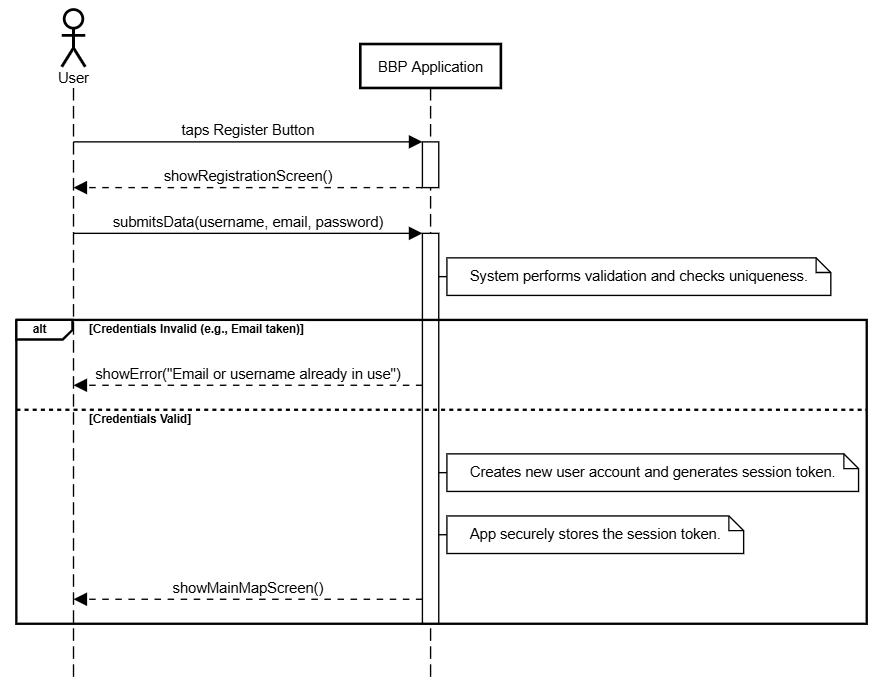
\includegraphics[width=1\linewidth]{RASD/LaTeXCode/images/sequenceDiagrams/UC_1.png}
        \caption{UC1}
        \label{fig:signup_as_ED_seqd}%
    \end{center}
\end{figure}

\subsubsection*{[UC\cuc]. Log In}
\begin{center}
    \begin{longtable}{|l|p{0.75\linewidth}|}
        \hline
        \textbf{Actor}            & Anonymous User \\
        \hline
        \textbf{Entry conditions} & The user is anonymous and is on a screen with a "Log In" option. \\
        \hline
        \textbf{Event Flow}       & 1 - BBP shows the login form. \\
                                  & 2 - The User inserts their username (or email) and password. \\
                                  & 3 - The User taps the "Log In" button. \\
                                  & 4 - BBP checks the credentials against the database. \\
                                  & 5 - BBP authenticates the user and creates an access session. \\
        \hline
        \textbf{Exit condition}   & The user is authenticated as a Registered User and is redirected to the main map screen. \\
        \hline
        \textbf{Exceptions}       & \begin{itemize}[noitemsep, nolistsep]
                                    \item The provided credentials (username/password) are incorrect. An error message is shown, and the user remains on the login page.
                                  \end{itemize}\\
        \hline
        \caption{Log In use case.}
        \label{tab:uc_login}
    \end{longtable}
\end{center}

\begin{figure}[H]
    \begin{center}
        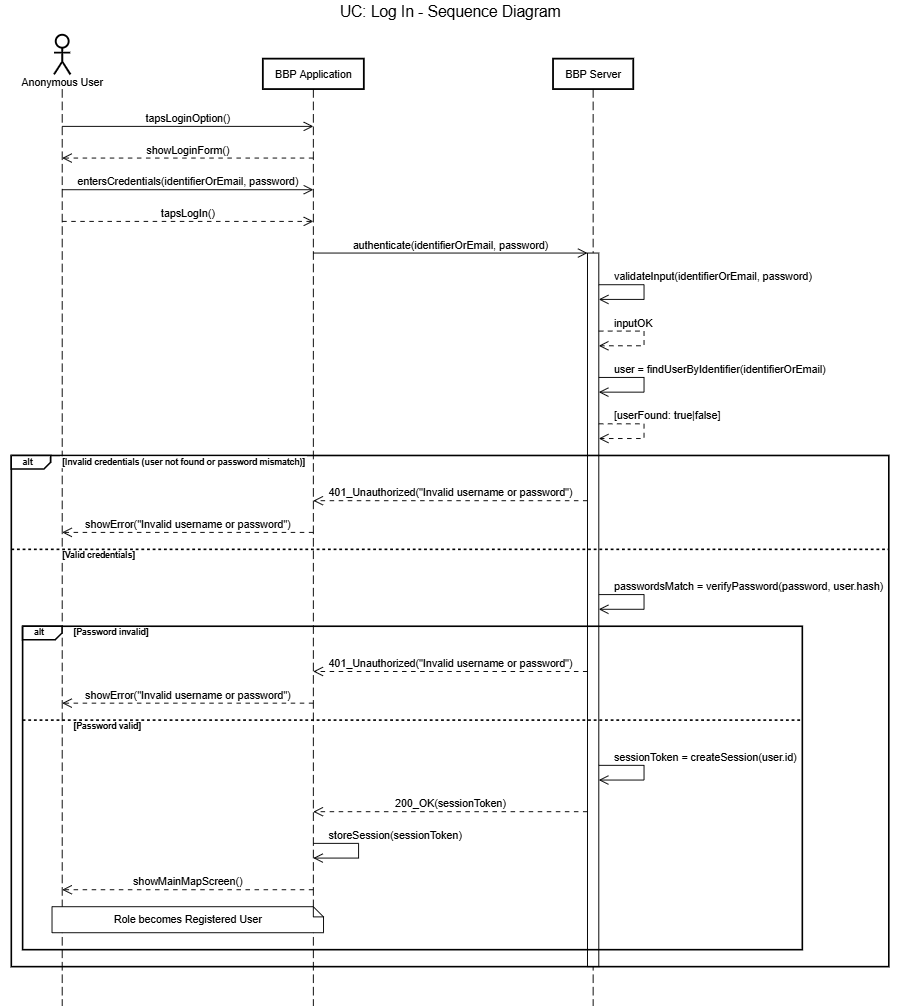
\includegraphics[width=1\linewidth]{RASD/LaTeXCode/images/sequenceDiagrams/UC_2.png}
        \caption{UC2}
        \label{fig:signup_for_registered_User}%
    \end{center}
\end{figure}


\subsubsection*{UC3. Log Out}
\begin{center}
    \begin{longtable}{|l|p{0.75\linewidth}|}
        \hline
        \textbf{Actor}            & Registered User \\
        \hline
        \textbf{Entry conditions} & The user is currently authenticated (logged in) in the BBP system. \\
        \hline
        \textbf{Event Flow}       & 1 - The User navigates to their profile or settings menu. \\
                                  & 2 - The User taps the "Log Out" button. \\
                                  & 3 - BBP invalidates and terminates the user's session. \\
                                  & 4 - BBP redirects the user to the main map screen (now as an Anonymous User). \\
        \hline
        \textbf{Exit condition}   & The user's session is terminated, and they are now an Anonymous User. \\
        \hline
        \textbf{Exceptions}       & \begin{itemize}[noitemsep, nolistsep]
                                    \item None.
                                  \end{itemize}\\
        \hline
        \caption{Log Out use case.}
        \label{tab:uc_logout}
    \end{longtable}
\end{center}
\begin{figure}[H]
    \begin{center}
        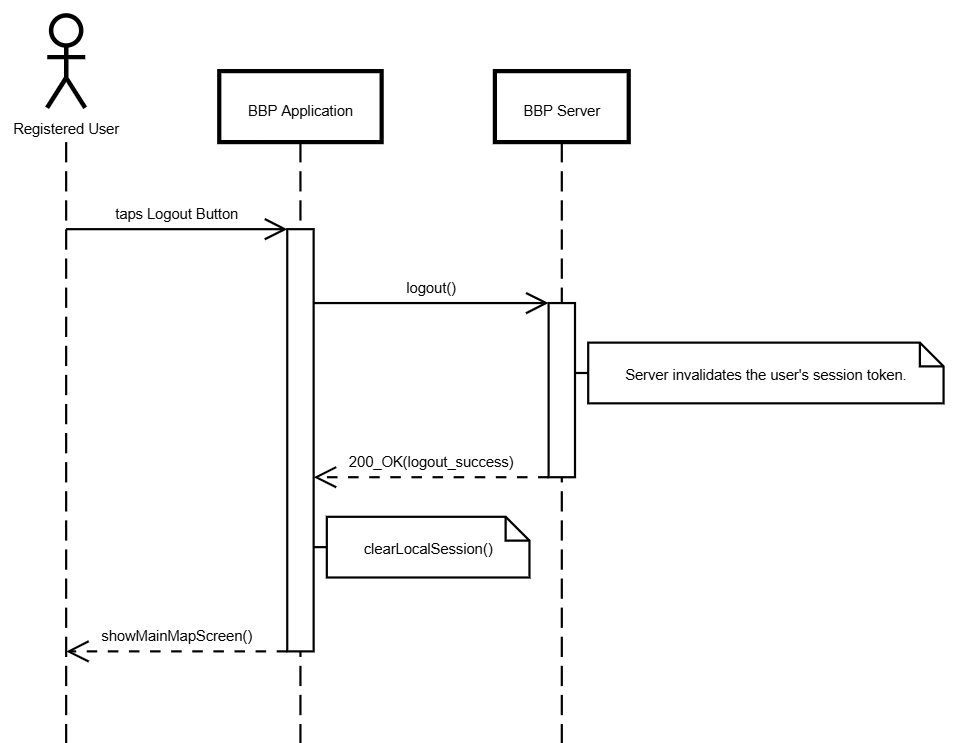
\includegraphics[width=1\linewidth]{RASD/LaTeXCode/images/sequenceDiagrams/UC_3.png}
        \caption{UC1.}
        \label{fig:UC3: Log Out - Sequence Diagram}%
    \end{center}
\end{figure}
%Use Cases Diagram for RCY
\subsubsection*{UC4. Search Paths}
\begin{center}
    \begin{longtable}{|l|p{0.75\linewidth}|}
        \hline
        \textbf{Actor}            & User (Anonymous or Registered), External Weather Service \\
        \hline
        \textbf{Entry conditions} & The user is on the main screen of the application. \\
        \hline
        \textbf{Event Flow}       & 1 - The User enters an origin and a destination in the search bar. \\
                                  & 2 - The User taps the "Search" button. \\
                                  & 3 - BBP sends the query to the Server. \\
                                  & 4 - The Server identifies all relevant public \texttt{Path}s. \\
                                  & 5 - For each path, the Server retrieves all associated \texttt{Status\_report} and \texttt{Obstacle\_report} instances. \\
                                  & 6 - The Server applies the merging logic (freshness, majority) to calculate the `derivedStatus` for each path . \\
                                  & 7 - The Server applies the scoring logic to calculate the `derivedScore` for each path . \\
                                  & 8 - The Server queries the \texttt{External Weather Service} for forecast data for the relevant locations . \\
                                  & 9 - The Server returns the list of paths, ordered by score, including their status and weather info. \\
                                  & 10 - BBP displays the ordered list of routes to the User. \\
        \hline
        \textbf{Exit condition}   & The user is presented with a list of matching paths ordered by score, or a "No results" message. \\
        \hline
        \textbf{Exceptions}       & \begin{itemize}[noitemsep, nolistsep]
                                    \item No paths are found matching the query. The system displays a "No results found" message.
                                    \item The \texttt{External Weather Service} is unavailable. Paths are shown without weather data, and a "Weather unavailable" message is displayed.
                                  \end{itemize}\\
        \hline
        \caption{Search Paths use case.}
        \label{tab:uc_search_paths}
    \end{longtable}
\end{center}
\begin{figure}[H]
    \begin{center}
        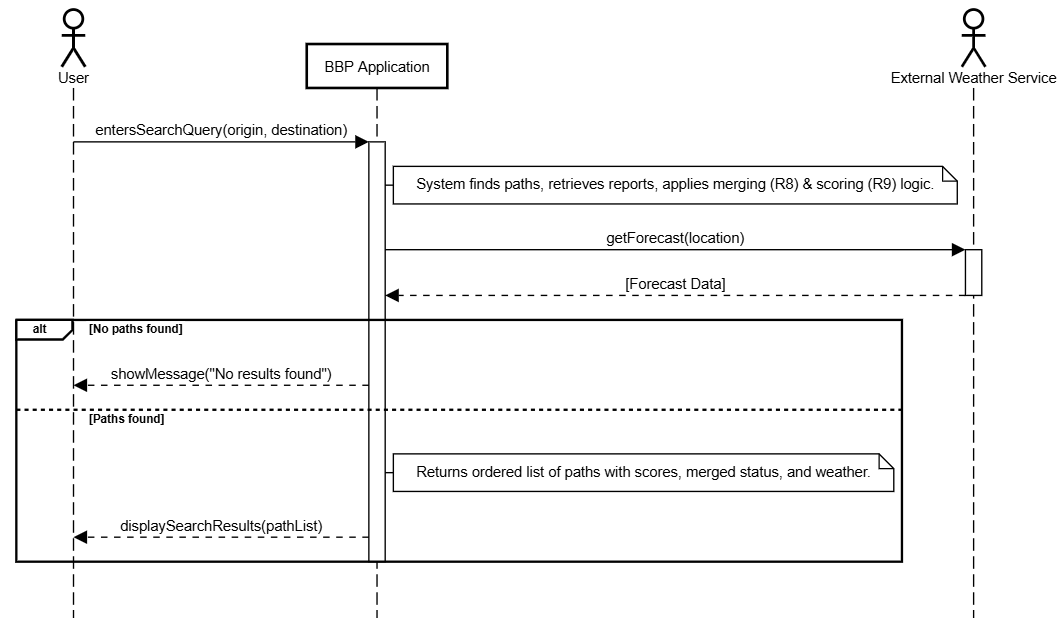
\includegraphics[width=1\linewidth]{RASD/LaTeXCode/images/sequenceDiagrams/UC_4.png}
        \caption{UC1.}
        \label{fig:UC4- Search Paths}%
    \end{center}
\end{figure}
\subsubsection*{UC5. View Path Details}
\begin{center}
    \begin{longtable}{|l|p{0.75\linewidth}|}
        \hline
        \textbf{Actor}            & User (Anonymous or Registered), External Weather Service \\
        \hline
        \textbf{Entry conditions} & The user is viewing a list of search results (\texttt{pathList}) from UC4. \\
        \hline
        \textbf{Event Flow}       & 1 - The User taps on a specific path from the results list. \\
                                  & 2 - BBP Application sends the selected \texttt{pathID} to the Server. \\
                                  & 3 - The Server retrieves the full details for the path, including its complete list of \texttt{GPS\_points}, all associated \texttt{Status\_report}s, and all \texttt{Obstacle\_report}s. \\
                                  & 4 - The Server applies the merging logic (R8) using the reports to calculate the definitive \texttt{derivedStatus}. \\
                                  & 5 - The Server queries the \texttt{External Weather Service} for an updated forecast (R13) . \\
                                  & 6 - The Server returns all path details (geometry, inclination, merged status, obstacles, weather) to the Application. \\
                                  & 7 - BBP Application displays the \texttt{Path Details} screen to the User. \\
        \hline
        \textbf{Exit condition}   & The user is viewing the detailed information for the selected path. \\
        \hline
        \textbf{Exceptions}       & \begin{itemize}[noitemsep, nolistsep]
                                    \item The selected \texttt{pathID} is invalid or no longer available. The system shows an error message.
                                    \item The \texttt{External Weather Service} is unavailable. Path details are shown without weather data.
                                  \end{itemize}\\
        \hline
        \caption{View Path Details use case.}
        \label{tab:uc_view_path_details}
    \end{longtable}
\end{center}
\begin{figure}[H]
    \begin{center}
        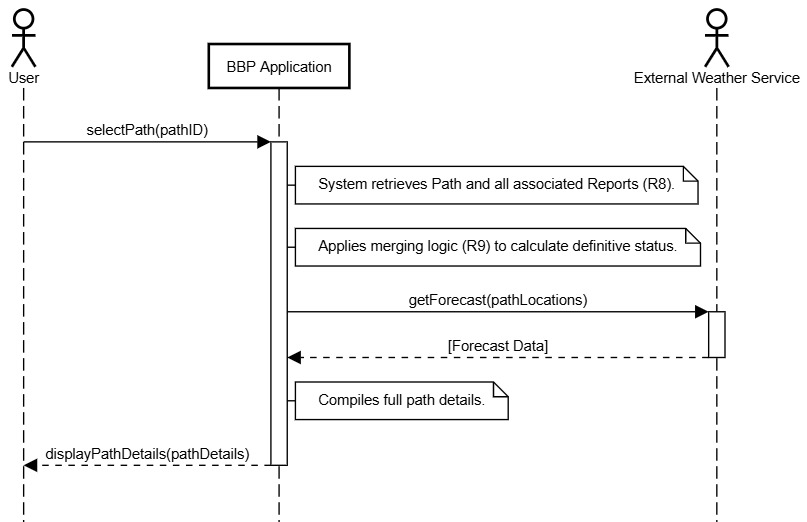
\includegraphics[width=1\linewidth]{RASD/LaTeXCode/images/sequenceDiagrams/UC_5.png}
        \caption{UC5 View Path Details}
        \label{fig:UC5: View Path Details}%
    \end{center}
\end{figure}
\subsubsection*{UC6. Follow Path (Navigation)}
\begin{center}
    \begin{longtable}{|l|p{0.75\linewidth}|}
        \hline
        \textbf{Actor}            & User (Anonymous or Registered), Device Sensors (GPS) \\
        \hline
        \textbf{Entry conditions} & The user is viewing the \texttt{Path Details} screen (from UC5). \\
        \hline
        \textbf{Event Flow}       & 1 - The User taps the "Follow Route" button. \\
                                  & 2 - BBP Application loads the path geometry (from the existing \texttt{Path}) onto the navigation screen. \\
                                  & 3 - BBP Application requests continuous location updates from the \texttt{Device Sensors} (GPS) [R15]. \\
                                  & 4 - The application displays the user's current location on the path route and calculates session statistics (time, distance, speed) . \\
                                  & 5 - \textbf{Note:} The app does not record the full geometry (it's already known) (R22, R23). \\
                                  & 6 - The User arrives at the destination (or manually taps "Stop Navigation"). \\
                                  & 7 - BBP Application stops the location updates and finalizes the session statistics. \\
                                  & 8 - BBP Application displays a "Summary" screen showing the session statistics (time, distance, avg speed). \\
                                  & 9 - \textbf{If User is Anonymous:} The Summary screen includes a "Register to Save" button (R16). \\
                                  & 10 - The Anonymous User taps "Register to Save", completes registration (UC1), selects a visibility (Public/Private), and the activity (stats-only) is saved (R18). \\
                                  & 11 - \textbf{If User is Registered:} The Summary screen includes a "Save Activity" button. \\
                                  & 12 - The Registered User taps "Save Activity", selects a visibility (Public/Private) , and the activity (stats-only) is saved to their archive. \\
                                  & 13 - If the user (Anonymous or Registered) exits the summary screen without saving/registering, the session data is discarded (R17). \\
        \hline
        \textbf{Exit condition}   & The user has completed navigation. The session activity (stats-only) is either saved with a visibility setting or discarded. \\
        \hline
        \textbf{Exceptions}       & \begin{itemize}[noitemsep, nolistsep]
                                    \item The user cancels navigation mid-way. The flow stops, stats are discarded, and the user is returned to the \texttt{Path Details} screen.
                                  \end{itemize}\\
        \hline
        \caption{Follow Path (Navigation) use case.}
        \label{tab:uc_follow_path}
    \end{longtable}
\end{center}
\begin{figure}[H]
    \begin{center}
        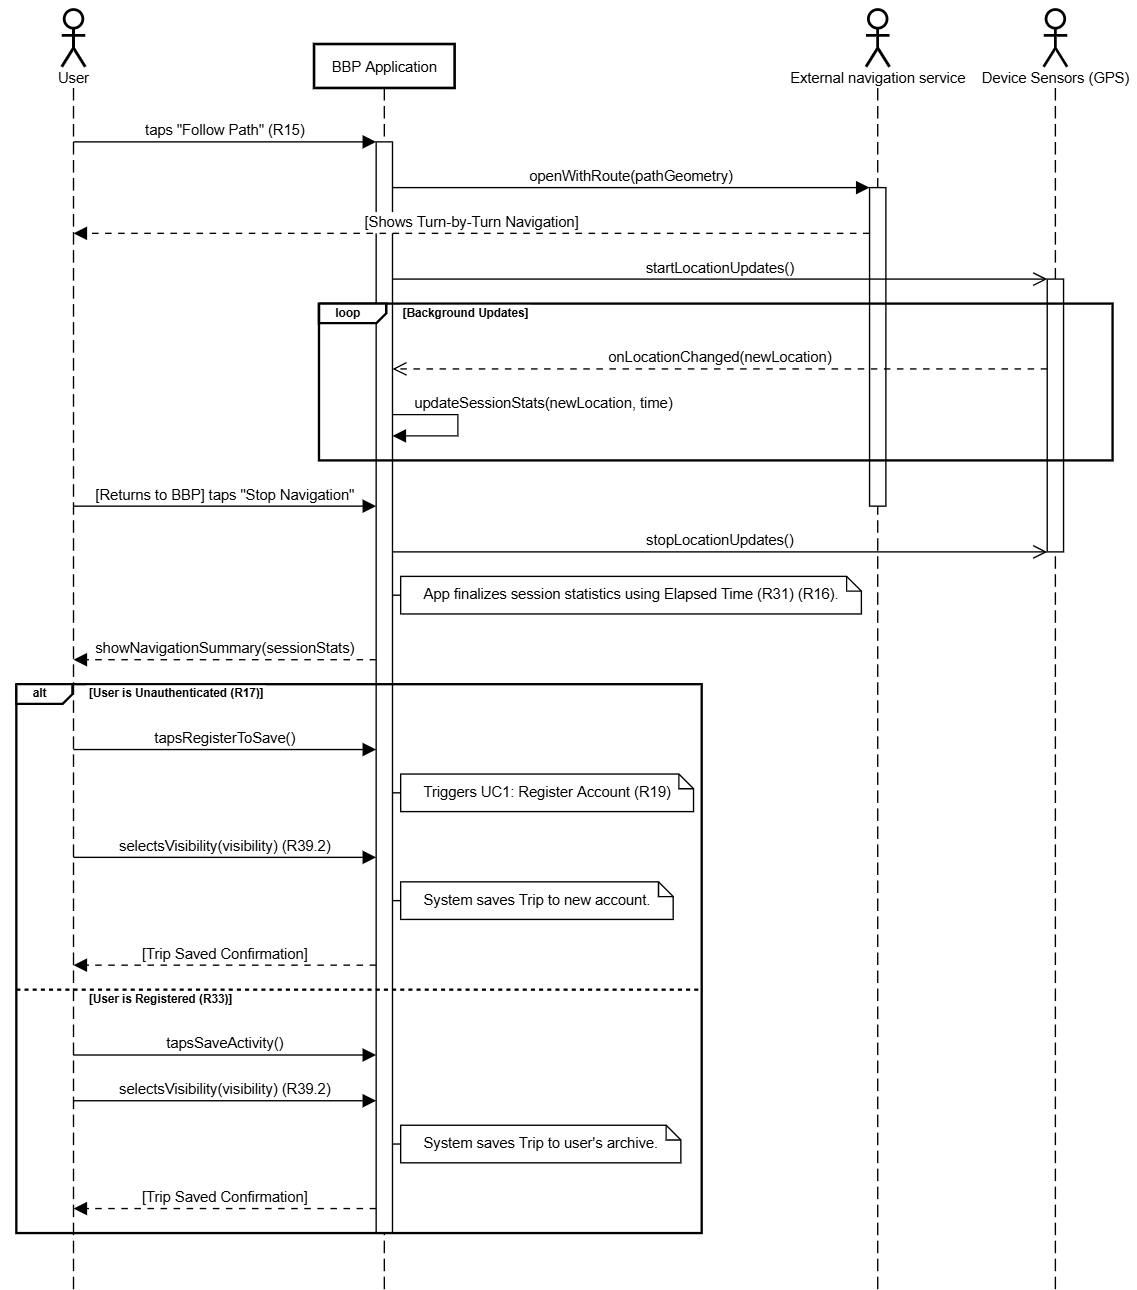
\includegraphics[width=0.65\linewidth]{RASD/LaTeXCode/images/sequenceDiagrams/UC_6.png}
        \caption{UC6: Follow Path (Navigation)}
        \label{fig:UC6: Follow Path}%
    \end{center}
\end{figure}
%Registred user activity
\subsubsection*{UC7. Record Path (Automatic)}
\begin{center}
    \begin{longtable}{|l|p{0.75\linewidth}|}
        \hline
        \textbf{Actor}            & Registered User, Device Sensors (GPS, IMU), External Weather Service \\
        \hline
        \textbf{Entry conditions} & The user is registered, logged in. (L'utente potrebbe aver selezionato un \texttt{Path} da seguire). \\
        \hline
        \textbf{Event Flow}       & 1 - The User taps the "Start Recording" button. \\
                                  & 2 - BBP Application activates \texttt{Device Sensors} [R22]. \\
                                  & 3 - The app displays the recording HUD, [R21]. \\
                                  & 4 - \textbf{In parallel:} The app records the user's \texttt{GPS\_points} sequence (R20) and monitors sensor data . \\
                                  & 5 - \textbf{If} sensor data exceeds the threshold, the app internally logs a new \texttt{sensor\_event} (R23) . \\
                                  & 6 - The User taps the "Stop Recording" button (R24). \\
                                  & 7 - BBP Application stops all sensors and finalizes the \texttt{Path} geometry. \\
                                  & 8 - BBP Application calculates the final \texttt{Statistics} (R28). \\
                                  & 9 - BBP show the summary of the new path with the trip information, and in case the \textit{ReviewDetections}. \textbf{`Save Trip and Path`} (UC9)\\
                                  
        \hline
        \textbf{Exit condition}   & The user has completed the recording. The system proceeds to the save flow (UC9). \\
        \hline
        \textbf{Exceptions}       & \begin{itemize}[noitemsep, nolistsep]
                                    \item The user discards the trip instead of saving. The recorded data is discarded.
                                  \end{itemize}\\
        \hline
        \caption{Record Trip (Automatic) use case.}
        \label{tab:uc_record_trip}
    \end{longtable}
\end{center}
\begin{figure}[H]
    \begin{center}
        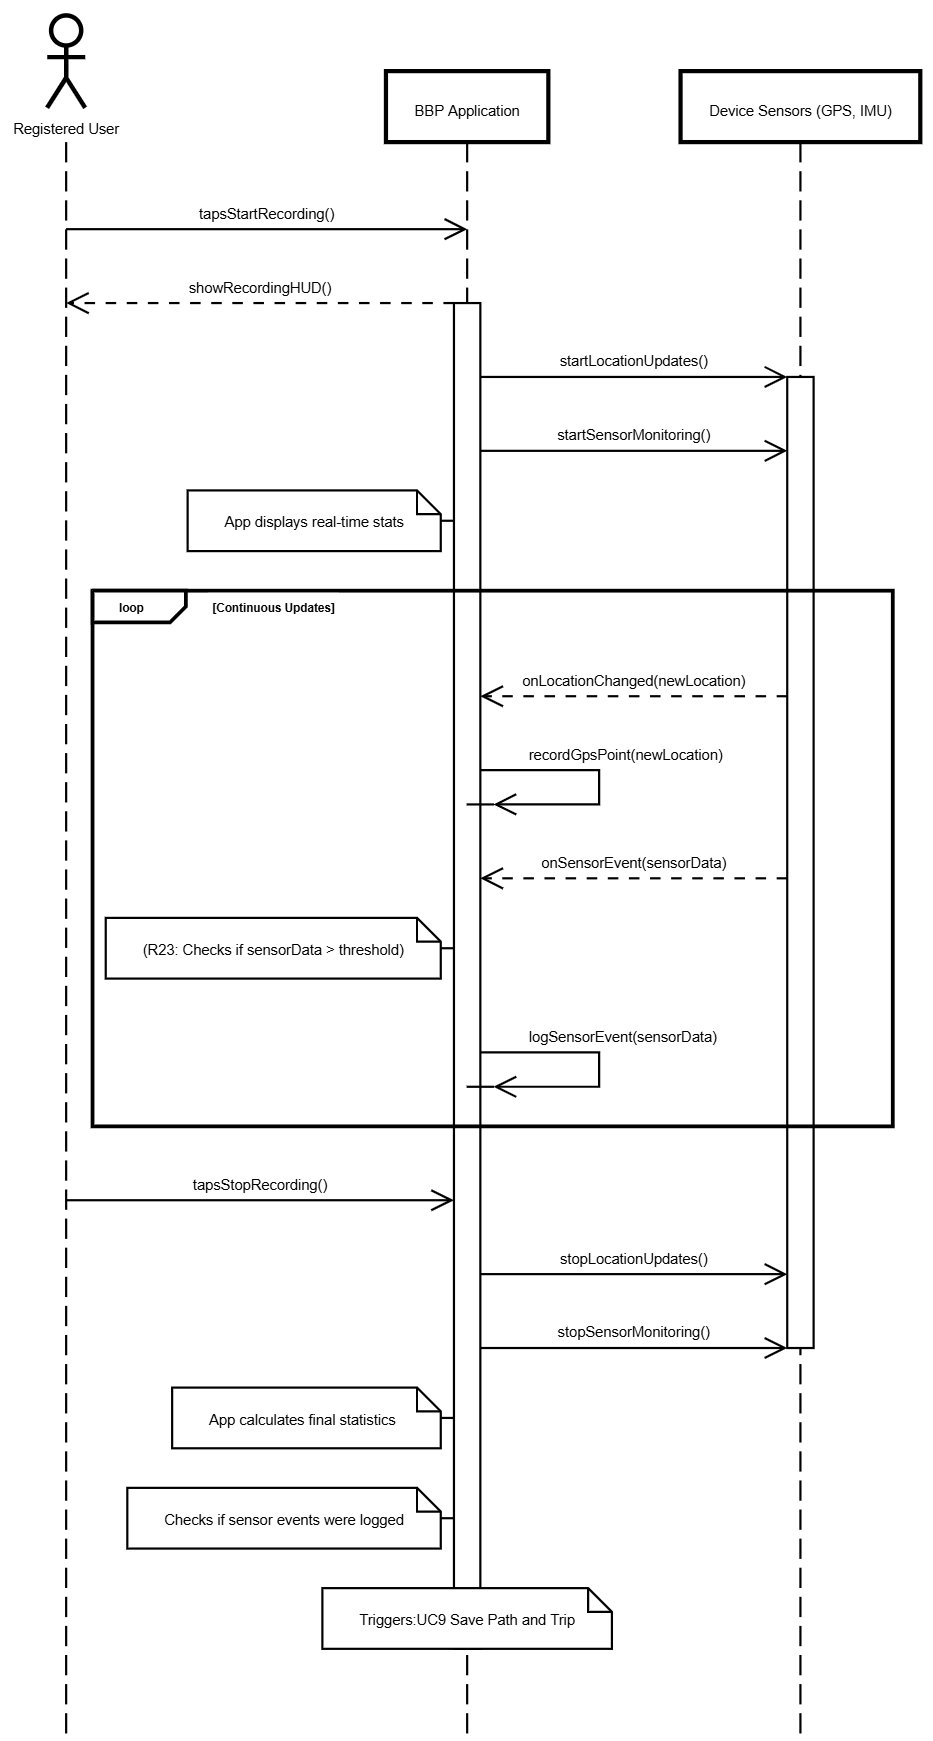
\includegraphics[width=0.75\linewidth]{RASD/LaTeXCode/images/sequenceDiagrams/UC_7.png}
        \caption{UC7: Record Trip }
        \label{fig:UC7: Record Trip }%
    \end{center}
\end{figure}
\subsubsection*{UC8. Review Detections}
\begin{center}
    \begin{longtable}{|l|p{0.75\linewidth}|}
        \hline
        \textbf{Actor}            & Registered User \\
        \hline
        \textbf{Entry conditions} & The user has just entered \texttt{Save Path and Trip} (UC9). \\
                                  & The system has logged one or more \texttt{sensor\_event}s (R25). \\
        \hline
        \textbf{Event Flow}       & 1 - The BBP Application displays the summary with the \texttt{Review Detections} screen. \\
                                  & 2 - The app shows the recorded path on a map, with pins marking the location of each logged \texttt{sensor\_event}. \\
                                  & 3 - The user reviews each detection (e.g., by tapping the pin). \\
                                  & 4 - For each event, the User chooses "Confirm" or "Ignore" (R26). \\
                                  & 5 - \textbf{If} "Confirm" is pressed, the system flags the \texttt{sensor\_event} as confirmed, ready to become an \texttt{Obstacle\_report} (R27). \\
                                  & 6 - \textbf{If} "Ignore" is pressed, the system flags the \texttt{sensor\_event} as rejected. \\
        \hline
        \textbf{Exit condition}   & All pending \texttt{sensor\_event}s have been processed. The system proceeds to the \texttt{Save Path and Trip} (UC9) decision. \\
        \hline
        \textbf{Exceptions}       & \begin{itemize}[noitemsep, nolistsep]
                                    \item The user exits the review screen prematurely. The system may treat all pending detections as "Ignored".
                                  \end{itemize}\\
        \hline
        \caption{Review Detections use case.}
        \label{tab:uc_review_detections}
    \end{longtable}
\end{center}
\begin{figure}[H]
    \begin{center}
        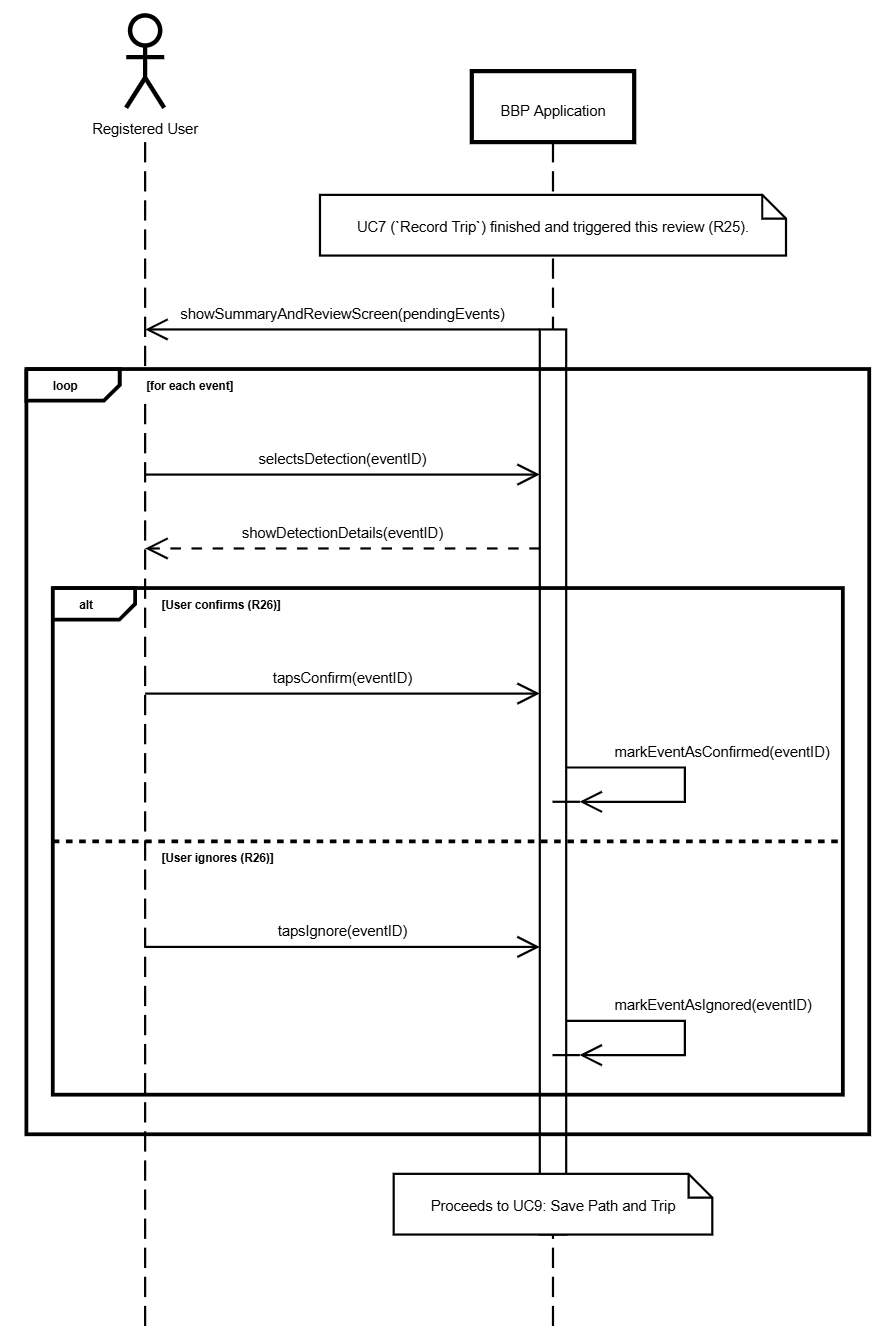
\includegraphics[width=1\linewidth]{RASD/LaTeXCode/images/sequenceDiagrams/UC_8.png}
        \caption{UC8: Review Detections}
        \label{fig:UC8: Review Detections}%
    \end{center}
\end{figure}
\subsubsection*{UC9. Save trip and path}
\begin{center}
    \begin{longtable}{|l|p{0.75\linewidth}|}
        \hline
        \textbf{Actor}            & Registered User \\
        \hline
        \textbf{Entry conditions} & The user has just completed \texttt{Record Trip (Automatic)} (UC7). \\
                                  & The application has the complete recorded data (geometry, stats, weather, and pending \texttt{sensor\_event}s). \\
        \hline
        \textbf{Event Flow}       & 1 - (Triggered by UC7) BBP Application displays the "Summary \& Save" screen, showing the map, final statistics (R28), and weather (R29). \\
                                  & 2 - \textbf{Extension Point `Review Detections` (UC8):} \textbf{If} pending \texttt{sensor\_event}s exist (R25), the flow is extended by UC8, prompting the user to confirm/ignore detections . \\
                                  & 3 - The User enters a name for the activity. \\
                                  & 4 - \textbf{`<<include>>` `set visibility` (UC12):} The User selects the visibility for the \textbf{`Trip` (Public/Private for stats} and for the \textbf{`Path` (Public/Private for search) [R39]} \\
                                  & 5 - The User taps "Save" or "Discard". \\
                                  & 6 - \textbf{If} "Save" is pressed: \\
                                  & \hspace{1em} a. BBP Application sends all finalised data (geometry, stats, weather, confirmed reports, name, visibilities) to the Server. \\
                                  & \hspace{1em} b. The Server saves the \texttt{Trip} to the user's private archive (R31). \\
                                  & \hspace{1em} c. The Server saves the \texttt{Path} with its chosen visibility (R39). \\
                                  & \hspace{1em} d. \textbf{If} the \texttt{Trip} visibility was "Public", the Server updates the \texttt{Path}'s average statistics (R8, R9). \\
                                  & 7 - \textbf{If} "Discard" is pressed, the flow terminates and data is deleted. \\
        \hline
        \textbf{Exit condition}   & The new \texttt{Trip} is saved. The new/updated \texttt{Path} is saved. Or all data is discarded. \\
        \hline
        \textbf{Exceptions}       & \begin{itemize}[noitemsep, nolistsep]
                                    \item Invalid data (e.g., missing name). The system shows an error and remains on the save screen.
                                  \end{itemize}\\
        \hline
        \caption{Save trip and path use case.}
        \label{tab:uc_save_trip_path}
    \end{longtable}
\end{center}
\begin{figure}[H]
    \begin{center}
        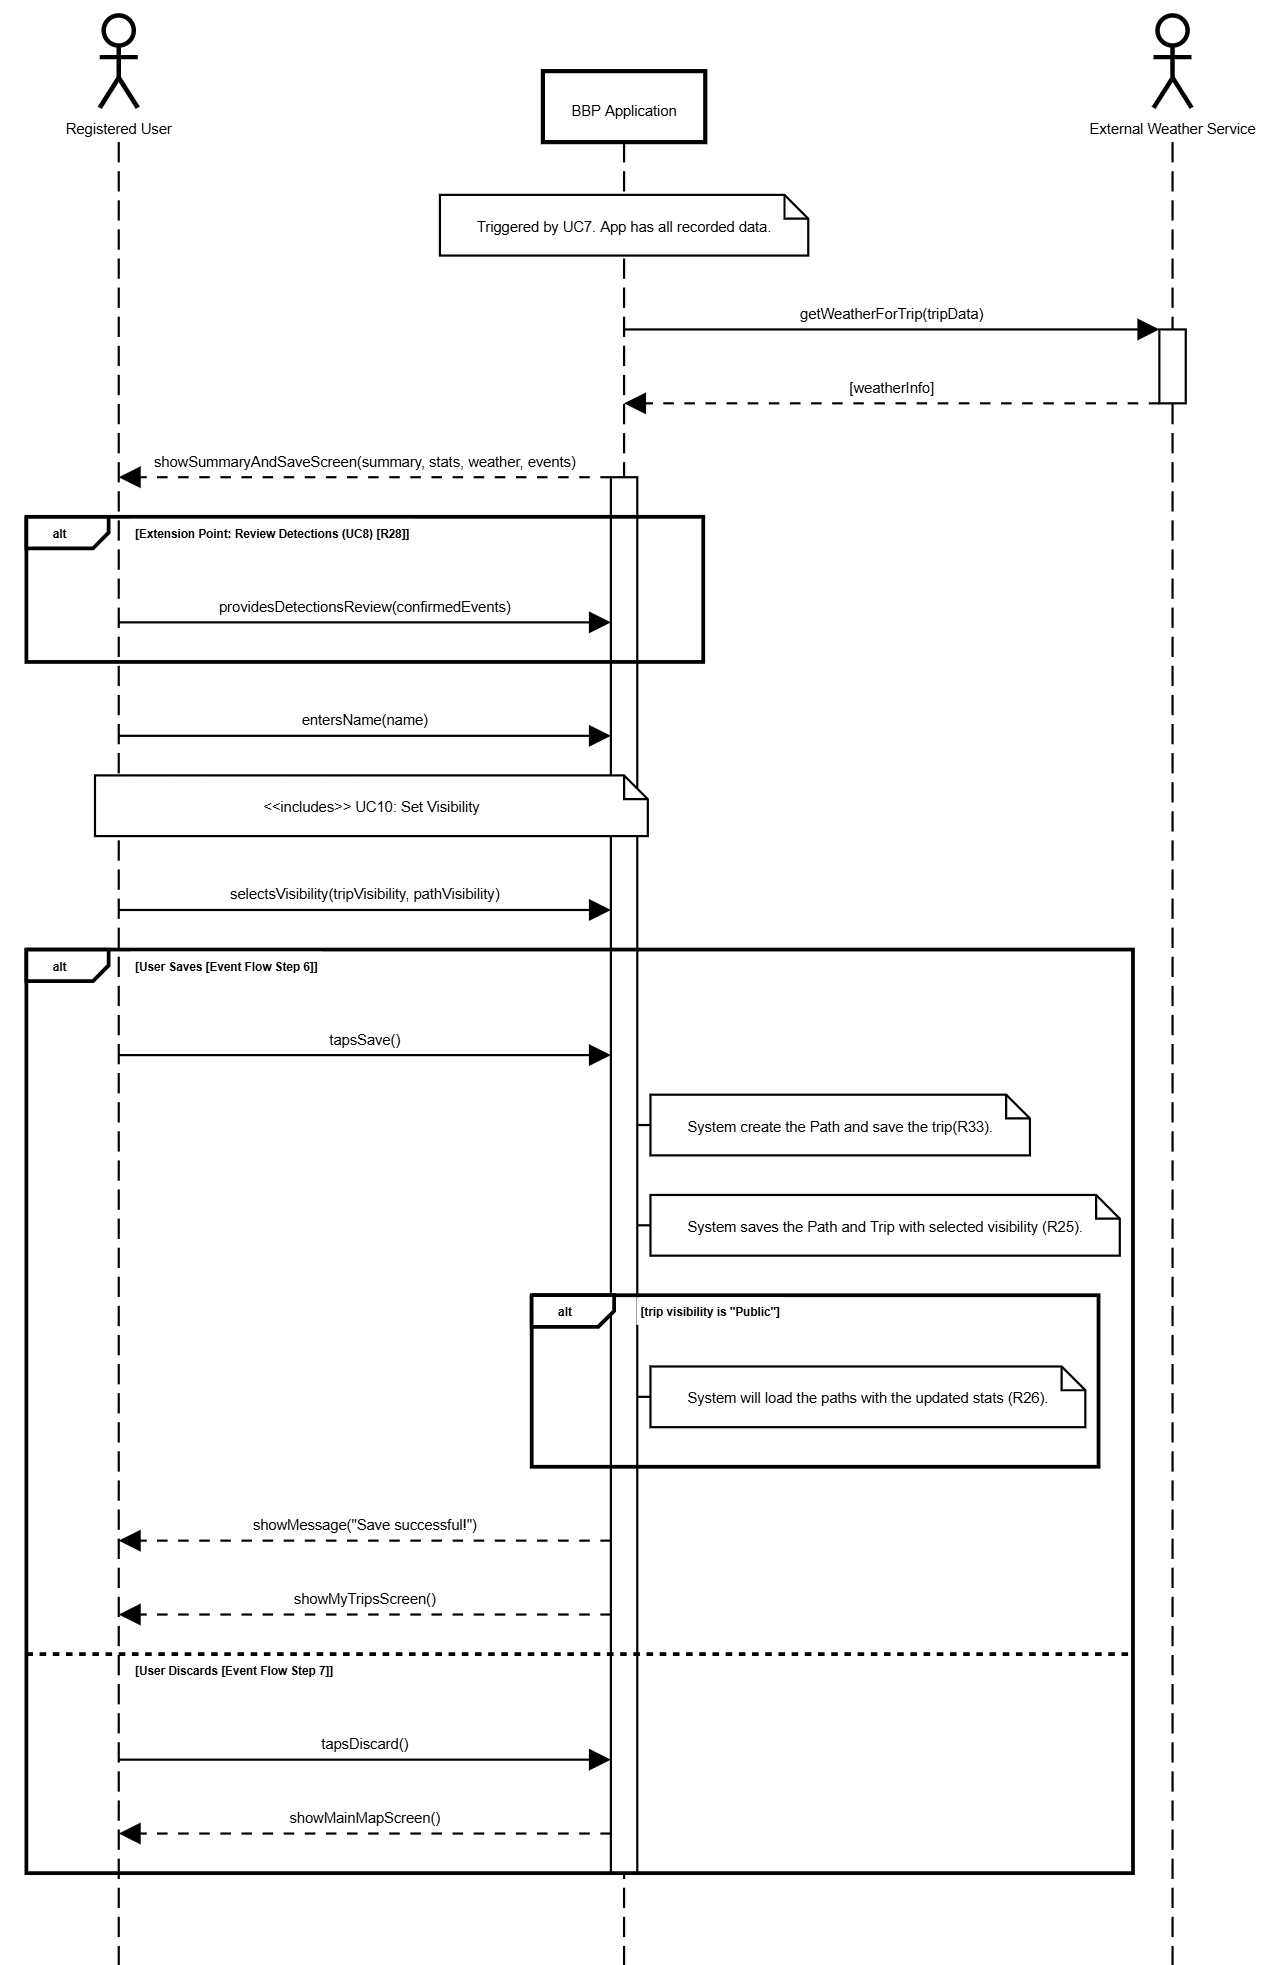
\includegraphics[width=1\linewidth]{RASD/LaTeXCode/images/sequenceDiagrams/UC_9.png}
        \caption{UC9: Save Path and Trip}
        \label{fig:UC9: Save Path and Trip}%
    \end{center}
\end{figure}
\subsubsection*{UC10. set visibility (Included)}
\begin{center}
    \begin{longtable}{|l|p{0.75\linewidth}|}
        \hline
        \textbf{Actor}            & Registered User \\
        \hline
        \textbf{Entry conditions} & The user is in the process of saving an activity (called by UC9 or UC12). \\
        \hline
        \textbf{Event Flow}       & 1 - (Triggered by UC9 or UC12) The system presents the User with the relevant visibility options [R39]. \\
                                  & 2 - \textbf{If} called by UC9 (\texttt{Save trip and path}), the User selects visibility for both the \texttt{Trip} (stats aggregation) and the \texttt{Path} (search). \\
                                  & 3 - \textbf{If} called by UC12 (\texttt{Save path}), the User selects visibility only for the \texttt{Path} (search). \\
                                  & 4 - The User confirms the selection. \\
        \hline
        \textbf{Exit condition}   & The visibility preference(s) are set and returned to the calling use case. \\
        \hline
        \textbf{Exceptions}       & \begin{itemize}[noitemsep, nolistsep]
                                    \item None. A default selection (e.g., "Private") is assumed.
                                  \end{itemize}\\
        \hline
        \caption{set visibility (Included) use case.}
        \label{tab:uc_set_visibility}
    \end{longtable}
\end{center}
\begin{figure}[H]
    \begin{center}
        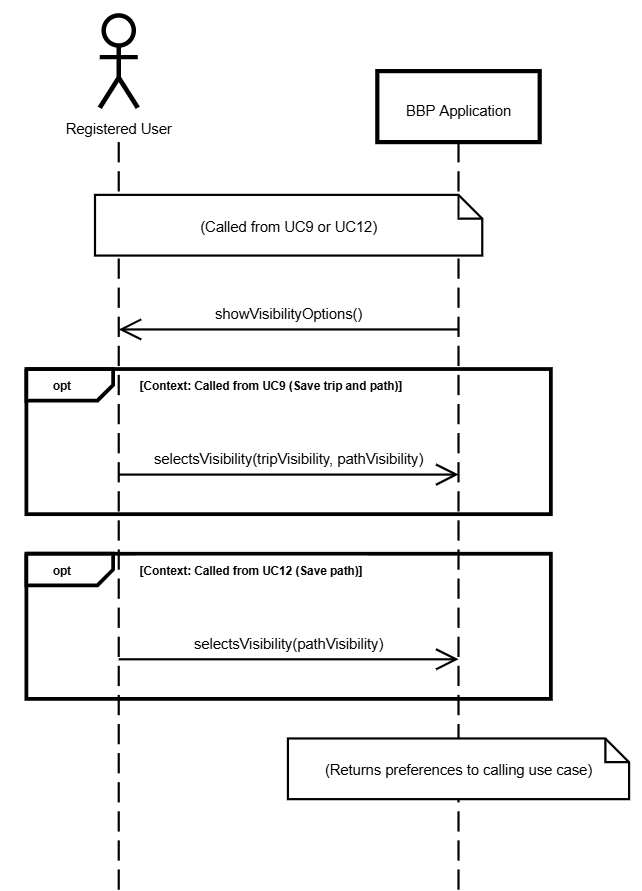
\includegraphics[width=1\linewidth]{RASD/LaTeXCode/images/sequenceDiagrams/UC_10.png}
        \caption{UC10: set visibility}
        \label{fig:UC10: set visibility}%
    \end{center}
\end{figure}
\subsubsection*{UC11. Create path manually}
\begin{center}
    \begin{longtable}{|l|p{0.75\linewidth}|}
        \hline
        \textbf{Actor}            & Registered User \\
        \hline
        \textbf{Entry conditions} & The user is registered, logged in, and has selected the "Create Path Manually" option. \\
        \hline
        \textbf{Event Flow}       & 1 - BBP Application displays the manual route editor screen, showing a map. \\
                                  & 2 - The User iteratively draws the path geometry by placing points on the map (R36). \\
                                  & 3 - The User taps "Done" or "Finish" when the path geometry is complete. \\
                                  & 4 - The system proceeds to the \textbf{`Save path`} use case (UC12), passing the new path data. \\
        \hline
        \textbf{Exit condition}   & The user has finished creating the path geometry. The system proceeds to the save flow (UC12). \\
        \hline
        \textbf{Exceptions}       & \begin{itemize}[noitemsep, nolistsep]
                                    \item The user cancels creation mid-way. The unsaved path data is discarded.
                                  \end{itemize}\\
        \hline
        \caption{Create path manually use case.}
        \label{tab:uc_create_path_manually}
    \end{longtable}
\end{center}
\begin{figure}[H]
    \begin{center}
        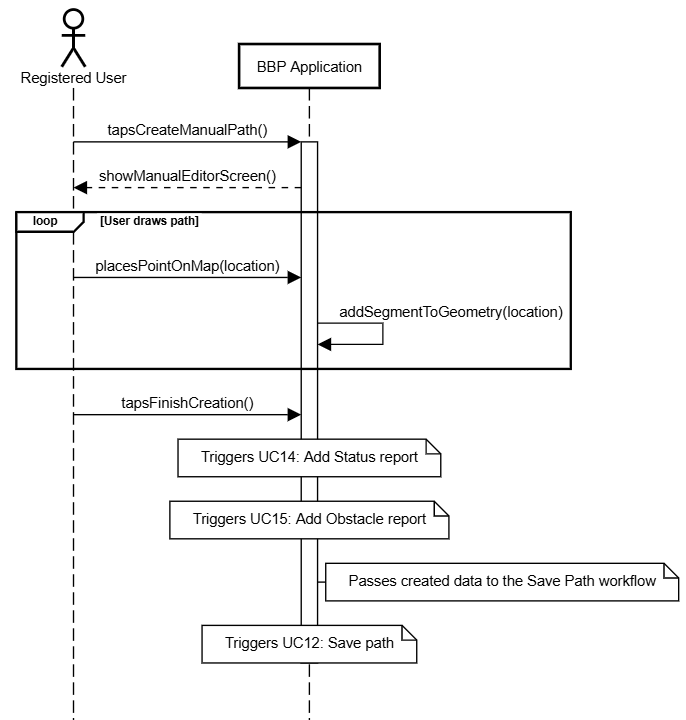
\includegraphics[width=1\linewidth]{RASD/LaTeXCode/images/sequenceDiagrams/UC_11.png}
        \caption{UC11. Create path manually}
        \label{fig:UC11. Create path manually}%
    \end{center}
\end{figure}
\subsubsection*{UC12. Save path}
\begin{center}
    \begin{longtable}{|l|p{0.75\linewidth}|}
        \hline
        \textbf{Actor}            & Registered User \\
        \hline
        \textbf{Entry conditions} & The user has just completed \texttt{Create path manually} (UC11). \\
                                  & The application has the new path geometry and any manual reports. \\
        \hline
        \textbf{Event Flow}       & 1 - (Triggered by UC11) BBP Application displays the "Save Path" screen. \\
                                  & 2 - The User enters a name for the \texttt{Path}. \\
                                  & 3 - \textbf{`<<include>>` `set visibility` (UC12):} The User selects the visibility for the \textbf{`Path`} (e.g., "Public" or "Private") [R39]. \\
                                  & 4 - The User taps "Save" or "Discard". \\
                                  & 5 - \textbf{If} "Save" is pressed: \\
                                  & \hspace{1em} a. BBP Application sends all finalized data (geometry, name, visibility) to the Server. \\
                                  & \hspace{1em} b. The Server saves the new \texttt{Path} with its chosen visibility (R39). \\
                                  & 6 - \textbf{If} "Discard" is pressed, the flow terminates and data is deleted. \\
        \hline
        \textbf{Exit condition}   & The new \texttt{Path} is saved with the chosen visibility, or all data is discarded. \\
        \hline
        \textbf{Exceptions}       & \begin{itemize}[noitemsep, nolistsep]
                                    \item Invalid data (e.g., missing name). The system shows an error and remains on the save screen.
                                  \end{itemize}\\
        \hline
        \caption{Save path use case.}
        \label{tab:uc_save_path}
    \end{longtable}
\end{center}
\begin{figure}[H]
    \begin{center}
        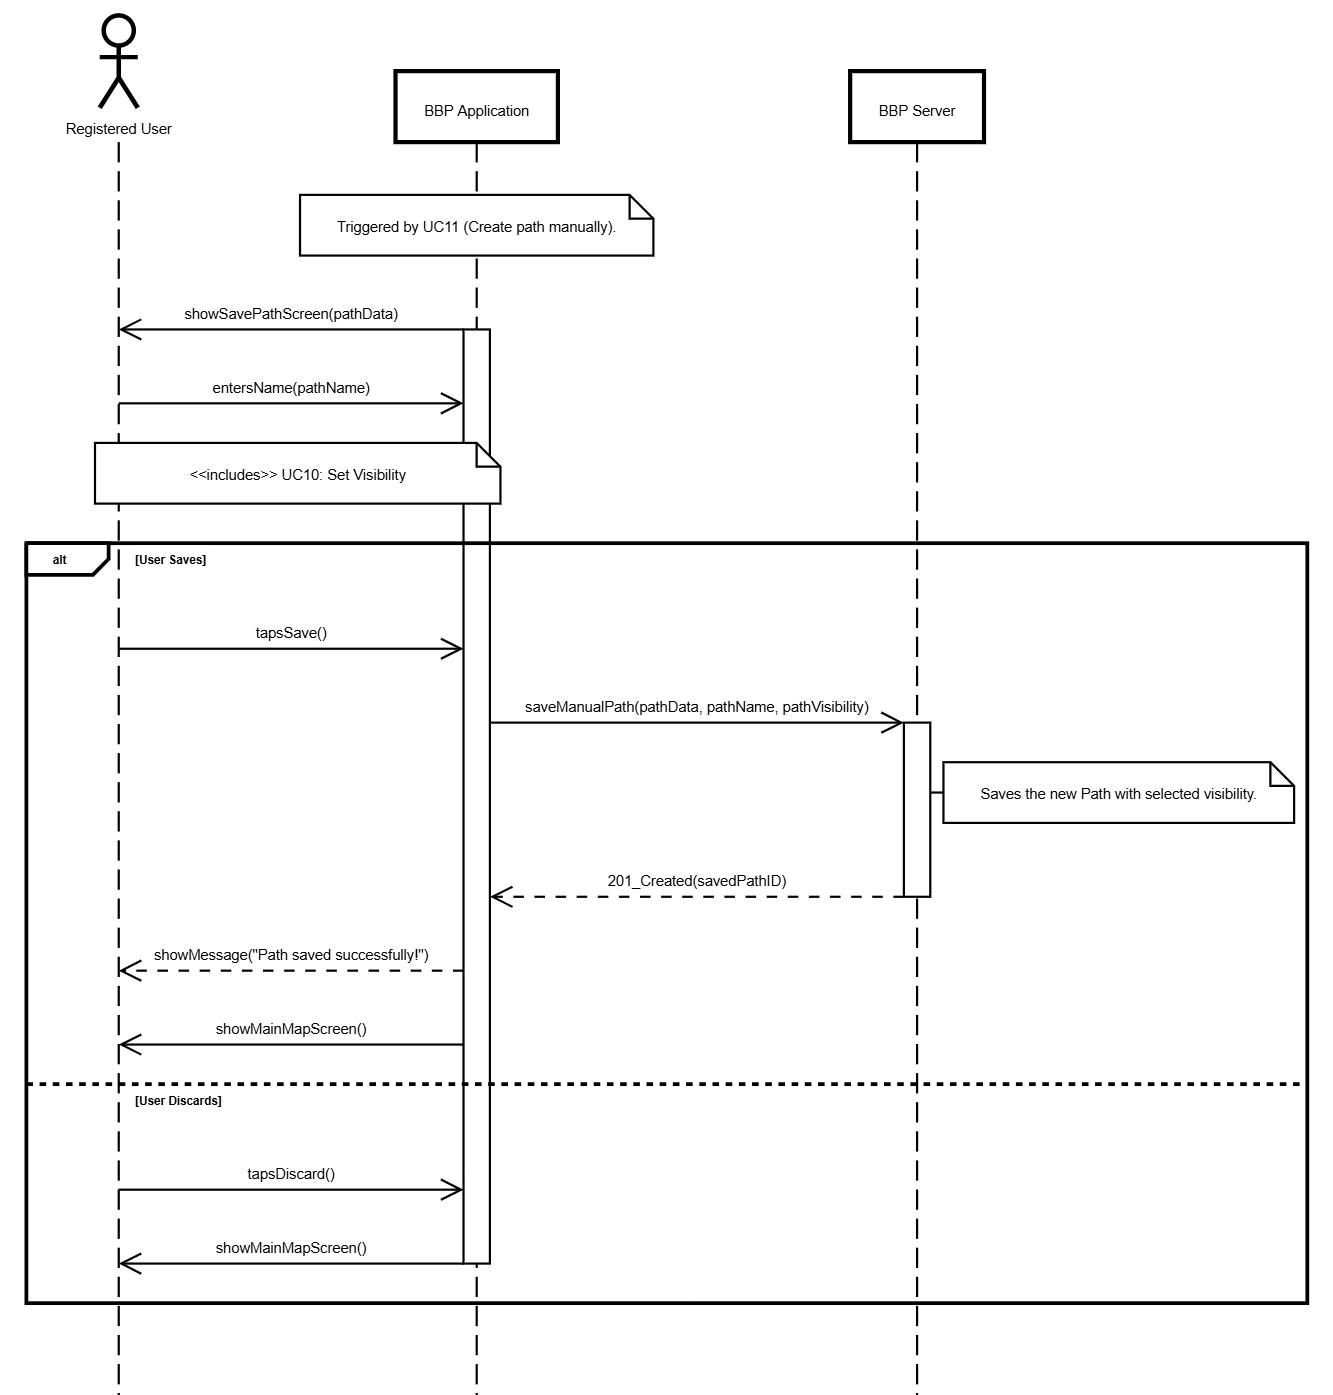
\includegraphics[width=1\linewidth]{RASD/LaTeXCode/images/sequenceDiagrams/UC_12.png}
        \caption{UC12: Save path}
        \label{fig:UC12: Save path}%
    \end{center}
\end{figure}

\begin{figure}[H]
    \begin{center}
        \includegraphics[width=.6\linewidth]{SequenceDiagrams/Evaluate a code v2.png}
        \caption{}
        \label{}%
    \end{center}
\end{figure}

\newpage



\begin{figure}[H]
    \begin{center}
        \includegraphics[width=.6\linewidth]{SequenceDiagrams/}
        \caption{}
        \label{}%
    \end{center}
\end{figure}

\newpage



\newpage

\subsection{Mapping on Goals}
\label{subsec:mapping_on_goals}

% Elenco dei Goals
\begin{itemize}
    \item \textbf{G1:} Support personal cycling activity tracking
    \item \textbf{G2:} Gather, aggregate, and provide users with actionable data regarding cycle path conditions
    \item \textbf{G3:} Facilitate the discovery and navigation of suitable cycling routes
    \item \textbf{G4:} Enhance trip analysis by enriching recorded user trips with relevant meteorological and physical data
    \item \textbf{G5:} Establish a community-based path evaluation system
\end{itemize}

% Goal G1
\subsubsection*{G1: Support personal cycling activity tracking}

\begin{table}[ht]
\centering
\caption{Goal G1: Support personal cycling activity tracking}
\label{tab:G1}
\begin{tabularx}{\textwidth}{|X|X|}
\hline
R1: BBP allows Users to sign up & D1: Users must have a mobile device (smartphone) equipped with GPS, accelerometer, and gyroscope sensors. \\ \hline
R2: BBP shall verify that the username and email provided during registration are not already in use. & D2: The device’s GPS sensor provides location data accurate enough to faithfully reconstruct the path taken. \\ \hline
R19: BBP shall provide feedback to the user in case of failed login attempts (e.g., incorrect credentials). & D7: Users act in good faith when providing manual data or confirming automatic detections. \\ \hline
\end{tabularx}
\end{table}

% Goal G2
\subsubsection*{G2: Gather, aggregate, and provide actionable data regarding cycle path conditions}

\begin{table}[ht]
\centering
\caption{Goal G2: Gather, aggregate, and provide actionable data regarding cycle path conditions}
\label{tab:G2}
\begin{tabularx}{\textwidth}{|X|X|}
\hline
\textbf{Requirement} & \textbf{Domain Assumption} \\ \hline
R7: BBP shall allow any user to search for public bike paths by specifying an origin and a destination. & D3: Accelerometer and gyroscope data correlate with real-world physical events (e.g., potholes, vibrations). \\ \hline
R9: BBP shall calculate a merged status for each searched path based on its associated Status_report instances. & D4: A data threshold exists to reliably distinguish significant movements (potholes) from normal biking vibrations. \\ \hline
\end{tabularx}
\end{table}

% Goal G3
\subsubsection*{G3: Facilitate the discovery and navigation of suitable cycling routes}

\begin{table}[ht]
\centering
\caption{Goal G3: Facilitate the discovery and navigation of suitable cycling routes}
\label{tab:G3}
\begin{tabularx}{\textwidth}{|X|X|}
\hline
\textbf{Requirement} & \textbf{Domain Assumption} \\ \hline
R14: BBP shall retrieve and display current weather forecast information for the selected path. & D12: The user, while cycling, will not change the track or get lost. \\ \hline
R15: BBP shall allow any user to select a path from the search results to view its details. & D14: Paths refer to either dedicated bike tracks or roads with low traffic and cycling-compatible speeds. \\ \hline
\end{tabularx}
\end{table}

% Goal G4
\subsubsection*{G4: Enhance trip analysis by enriching recorded user trips with relevant meteorological and physical data}

\begin{table}[ht]
\centering
\caption{Goal G4: Enhance trip analysis by enriching recorded user trips with relevant meteorological and physical data}
\label{tab:G4}
\begin{tabularx}{\textwidth}{|X|X|}
\hline
\textbf{Requirement} & \textbf{Domain Assumption} \\ \hline
R29: After recording, BBP shall retrieve and associate weather information with the trip. & D11: The external weather service API is available, stable, and provides accurate data. \\ \hline
\end{tabularx}
\end{table}

% Goal G5
\subsubsection*{G5: Establish a community-based path evaluation system}

\begin{table}[ht]
\centering
\caption{Goal G5: Establish a community-based path evaluation system}
\label{tab:G5}
\begin{tabularx}{\textwidth}{|X|X|}
\hline
\textbf{Requirement} & \textbf{Domain Assumption} \\ \hline
R36: BBP shall allow RCY to manually create paths on a map. & D8: “Fresh” (recent) information is considered more relevant than older data when describing a path’s status. \\ \hline
R37: BBP shall allow RCY to submit Status_reports manually for paths. & D9: Users provide correct and rational evaluations during path assessments. \\ \hline
\end{tabularx}
\end{table}




\section{Performance requirements}
\label{sec:performance_requirements}%
\paragraph{Number of concurrent Users:} 
\paragraph{Data storage:} 
\paragraph{Time response:} 


\newpage
\section{Design constraints}
\label{sec:design_constraints}%


\subsection{Standard compliance}
\label{subsec:standard compliance}%%


\subsection{Hardware limitations}
\label{subsec:hardware_limitations}%



\section{Software system attributes}
\label{sec:software_system_attributes}%

\subsection{Reliability}
\label{subsec:reliability}%
.

\subsection{Availability}
\label{subsec:availability}%


\subsection{Security}
\label{subsec:security}%



\subsection{Maintainability}
\label{subsec:maintainability}%


\subsection{Portability}
\label{subsec:portability}%



